\documentclass[a4paper,12pt,article]{memoir}
\usepackage{amsmath}
\usepackage{amssymb}
\usepackage{mathspec}
\usepackage{xltxtra}
\usepackage{polyglossia}
\usepackage{MnSymbol}
\usepackage{siunitx,cancel,graphicx}
\usepackage{enumitem}
\usepackage{hyperref,graphicx}
\usepackage{icomma}
\usepackage{float}
\usepackage{mleftright}

\usepackage{listings}
\usepackage{color}
\usepackage{xcolor}

\usepackage[
backend=biber,
style=numeric,
citestyle=numeric,
sorting=none
]{biblatex}
\addbibresource{resources.bib}


% This is the color used for MATLAB comments below
\definecolor{MyDarkGreen}{rgb}{0.0,0.4,0.0}
\definecolor{Blue}{rgb}{0.0,0.0,1.0}
\definecolor{Purple}{rgb}{1.0,0.0,1.0}

\colorlet{mygray}{black!30}
\colorlet{mygreen}{green!60!blue}
\colorlet{mymauve}{red!60!blue}

\lstset{
  backgroundcolor=\color{gray!10},
  basicstyle=\ttfamily,
  columns=fullflexible,
  breakatwhitespace=false,
  breaklines=true,
  captionpos=b,
  commentstyle=\color{mygreen},
  extendedchars=true,
  frame=single,
  keepspaces=true,
  keywordstyle=\color{blue},
  language=c++,
  numbers=none,
  numbersep=5pt,
  numberstyle=\tiny\color{blue},
  rulecolor=\color{mygray},
  showspaces=false,
  showtabs=false,
  stepnumber=5,
  stringstyle=\color{mymauve},
  tabsize=3,
  title=\lstname
}






\setdefaultlanguage{english}

\defaultfontfeatures{Scale=MatchLowercase,Mapping=tex-text}
%\setmainfont[Numbers=Lowercase]{Minion Pro}
%\setsansfont[Numbers=Lowercase]{Myriad Pro}
%\setmonofont{Menlo}
%\setmathsfont(Digits,Latin,Greek)[Numbers={Lining,Proportional}]{Minion Pro}

\sisetup{%
  output-decimal-marker = {,},
  per-mode = symbol,
  %round-mode = places,
  %round-precision = 5
}



\setlrmarginsandblock{2.5cm}{2.5cm}{*}
\setulmarginsandblock{1.5cm}{2cm}{*}
\checkandfixthelayout

\setlength{\parindent}{2em}
\setlength{\parskip}{0pt}

\newcommand{\f}{\fancybreak}

\DeclareSIUnit \electronvolt {\ensuremath{eV}}

\newcommand{\mvec}[2]{
\ensuremath{\left(
\begin{array}{c}
#1\\
#2\\
\end{array}
\right)}
}

\newcommand{\Span}{\ensuremath{\mathrm{Span}}}
\newcommand{\Mat}{\ensuremath{\mathrm{Mat}}}
\newcommand{\C}{\ensuremath{\mathbb{C}}}
\newcommand{\R}{\ensuremath{\mathbb{R}}}
\newcommand{\Rno}{\ensuremath{\mathbb{R}\backslash\{0\}}}
\newcommand{\Z}{\ensuremath{\mathbb{Z}}}
\newcommand{\ol}[1]{\ensuremath{\overline{#1} } }
\newcommand{\F}[1]{\ensuremath{\mathbb{F}_{#1} } }

\title{Abstract for student Colloquium}
\author{Nikolaj Roager Christensen, 201805275}
\date{\today} %

\begin{document}

\maketitle


\noindent Name: Nikolaj Roager Christensen (201805275)

\noindent Title: Simulating particles in electric and magnetic fields

\noindent Date and time for Student Colloquium: March 17, 2021

\noindent Supervisor: Dmitri Fedorov


\noindent Abstract:

In this Student Colloquium, I wish to demonstrate a numerical simulation of single classical particles in various magnetic and electric setups. The main goal is to show why charged particles will follow the magnetic field, even though the magnetic force on a particle is perpendicular to the direction of the field. As a starting point, I will re-create the well-known behaviour of particles in a constant magnetic field, then I will demonstrate how and why magnetic fields can concentrate or trap charged particles, using as examples toroidal coils, such as the ones in  Tokamak-style fusion reactors, I will also explain how this relates to the naturally occurring magnetic field of the Earth. Finally I will use my simulation to demonstrate a classical cyclotron particle accelerator, as an example of combined electric and magnetic setups.

\begin{center}
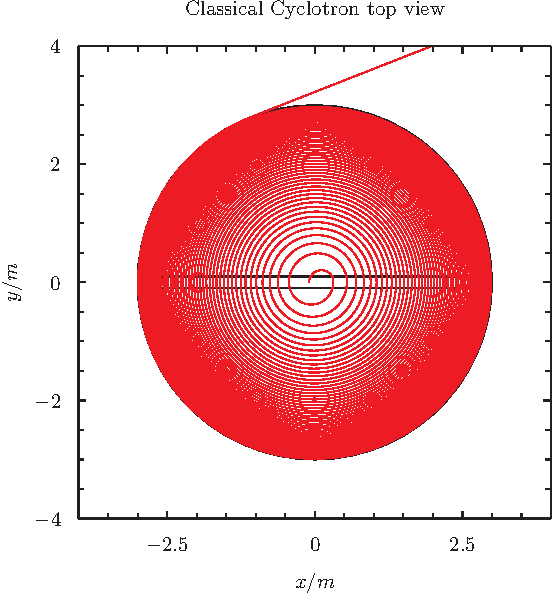
\includegraphics[width=0.8\linewidth]{cyclotron1_xy-view.pdf}

A plot of the path of a particle in a classical cyclotron, from my simulation. This will be included in the presentation, and is my personal pick for the front-page
\end{center}


\end{document}
